\section{Introduction}

% 第一段
Quantum error correction (QEC) is essential for building reliable and large-scale quantum computers \cite{terhal2015quantum}. QEC protects quantum information against noise by redundantly encoding logical qubits into multiple physical qubits \cite{calderbank1996good}. Quantum low-density parity-check (qLDPC) codes are a promising code. Unlike the commonly used surface code~\cite{fowler2012surface,bonilla2021xzzx}, which needs a quadratic number of physical qubits to encode logical qubits, qLDPC codes achieve a constant encoding rate and thus scale linearly in physical qubits. This high encoding rate makes qLDPC codes attractive for scalable fault-tolerant architectures. Recent work has further demonstrated the feasibility of implementing qLDPC codes on neutral-atom and superconducting platforms \cite{xu2024constant,bbcode,wang2025demonstration}. 

% 第二段
Beyond code design, the decoder is central to the QEC workflow \cite{vittal2023astrea,alavisamani2024promatch,das2022lilliput,wu2025micro}, since it identifies both the type and location of errors. A QEC cycle begins by encoding a logical qubit into an entangled state of many physical qubits~\cite{knill1997theory,laflamme1996perfect}. Repeated stabilizer measurements then extract syndromes (binary string) that capture the presence and location of physical errors without collapsing the logical state. The decoder interprets these syndromes to infer the underlying error configuration and determines the appropriate correction operator. As a result, decoder performance directly dictates the fault-tolerance capability of the entire quantum system.

% Beyond the design of QEC codes, the decoder plays a pivotal role in the overall QEC process \cite{vittal2023astrea,alavisamani2024promatch,das2022lilliput,wu2025micro}, which is used to detect the error type and its allocation. Specifically, a complete QEC cycle begins by encoding a logical qubit into an entangled state of multiple physical qubits~\cite{knill1997theory,laflamme1996perfect}. Then, the stabilizer measurements are repeatedly performed to detect errors on the physical qubits, without collapsing the logical quantum state. These measurements yield binary strings, known as syndromes, that imply the error information about the occurrence and location of physical errors. Consequently, the role of the decoder is to explicitly reveal the error type and location, allowing us to perform a suitable correction operator that compensates for the logical errors. Therefore, the performance of the decoder directly determines the overall fault tolerance of the quantum system.


%%%%%%%%%%%%%%%%%%%%%%%%%%%%%%%%%%%%%%%%%%

\begin{figure}[t]
\centerline{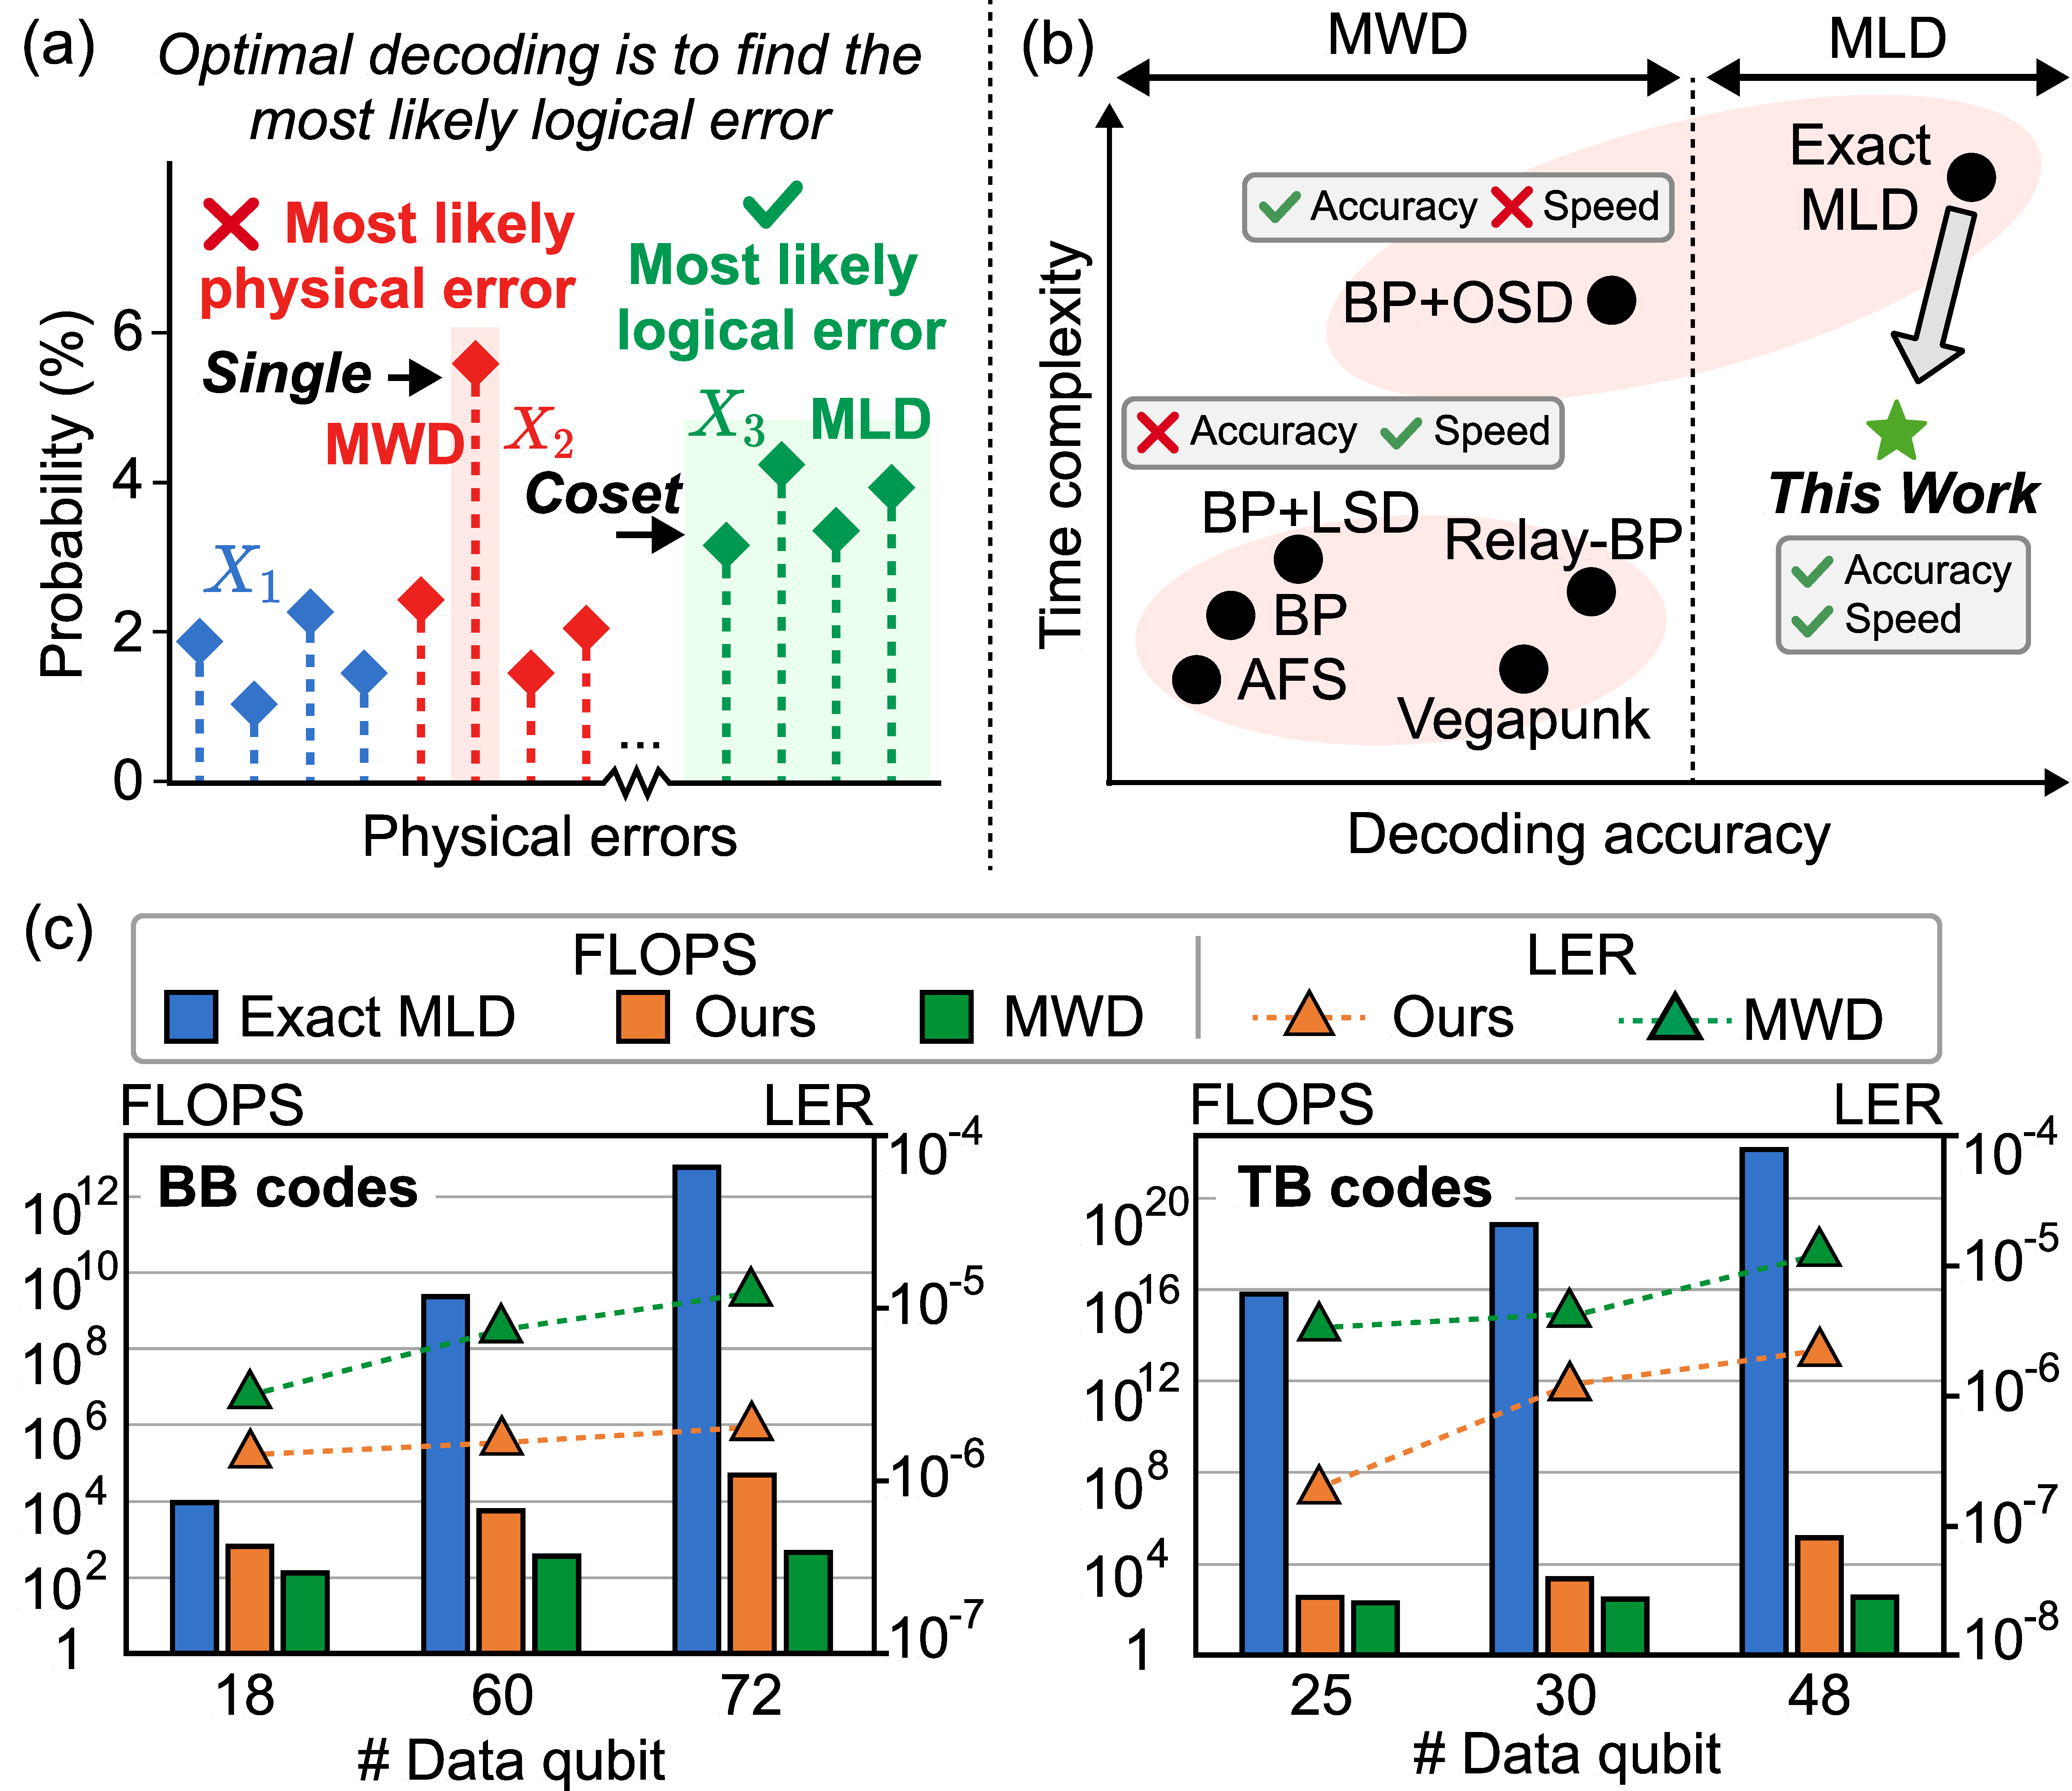
\includegraphics[width=1.0\columnwidth]{figures/intro.pdf}}
\vspace{-0.3cm}
\caption{(a) Difference between minimum weight decoding (MWD) and maximum likelihood decoding (MLD). MLD is optimal since it targets the most likely logical errors.
(b) Trade-off between decoding accuracy and time complexity of existing QEC decoders. They either have low accuracy or high time complexity.
(c) Computational cost (FLOPS) and logical error rate (LER) comparison among exact MLD, \papername, and MWD (BP+OSD) decoder.
} 
\label{fig:intro}
\end{figure}
%%%%%%%%%%%%%%%%%%%%%%%%%%%%%%%%%%%%%%%%%%



%%%%%%%%%%%%%%%%%%%%%%%%%%%%%%%%%%%%%%%%%%
% \begin{table}[t]
\centering
\renewcommand{\arraystretch}{1.2}
\caption{Comparison with other qLDPC decoders.}
\label{tab:intro_comparison}
\resizebox{\linewidth}{!}{
\begin{minipage}{\linewidth}
\begin{tabular}{|l|c|c|c|c|}
\toprule[1pt]
    \textbf{\makecell{Decoder Type}} & \textbf{\makecell{Decoding\\Accuracy}} & \textbf{\makecell{Time\\Complexity}} & \textbf{\makecell{Technical\\Feature}} & \textbf{Principle} \\
    \hline
    AFS \cite{das2022afs} & \bad & \good & \makecell{Union-find} & MWD \\
    \hline
    Astrea \cite{vittal2023astrea} & \good & \medium & \makecell{Graph\\Matching}  & MWD \\
    \hline
    BP \cite{bp} & \bad & \good & \makecell{Message\\Passing}  & MWD \\
    \hline
    BP+OSD \cite{bposd} & \good & \bad & \makecell{Gaussian\\Elimination}  & MWD \\
    \hline
    BP+LSD \cite{bplsd} & \medium & \medium & \makecell{Matrix\\Factorization}  & MWD \\
    \hline
    \textbf{\papername} & \good & \good & \makecell{Tensor\\Compression} & \textbf{MLD} \\
\bottomrule[1pt]
\end{tabular}

\vspace{0.15cm}
\raggedright
\footnotesize
$^*$MWD refers to Minimum Weight Decoding, while MLD means Maximum Likelihood Decoding. \\
$^*$The symbol $\odot$ indicates a medium level.
\end{minipage}
}
\vspace{-0.4cm}
\end{table}


%%%%%%%%%%%%%%%%%%%%%%%%%%%%%%%%%%%%%%%%%%

% 第三段
The design of a qLDPC decoder depends heavily on the target error model, which is typically categorized into \textit{the most likely physical error} and \textit{the most likely logical error}. The former is addressed by minimum-weight decoding (MWD), which selects the physical error with the lowest weight that is consistent with the syndrome. As shown in \autoref{fig:intro}~(a), MWD returns only a single most probable physical error ($\mathbf{X}_2$). In contrast, maximum-likelihood decoding (MLD) evaluates all physical errors within a coset and identifies the most probable logical error ($\mathbf{X}_3$), achieving globally optimal performance~\cite{sundaresan2023demonstrating,mld,jung2020quantum}. Due to quantum degeneracy, the true logical error corresponds to a large set of physical errors, making MWD inherently approximate and often inaccurate. In our experiments, even the state-of-the-art BP+OSD decoder~\cite{bposd} correctly compensates the true logical error with only 18.4\% probability on a 72-qubit bivariate bicycle (BB) code.

% The qLDPC decoder design highly depends on the target error type, which is generally categorized into \textit{the most likely physical error} and \textit{the most likely logical error}. The first one is followed by the minimum weight decoding algorithm (MWD) that minimizes the Hamming weight of the physical error vector while matching the observed syndrome. As illustrated in \autoref{fig:intro}~(a), MWD only identifies one single physical error with the highest probability ($\mathbf{X}_2$). In contrast, the maximum likelihood decoding algorithm (MLD) checks all physical errors and targets the most likely logical error ($\mathbf{X}_3$), achieving globally optimal decoding performance~\cite{sundaresan2023demonstrating,mld,jung2020quantum}. 
% Note that the presence of quantum degeneracy means that the true logical error corresponds to a large coset of possible physical errors. Consequently, the MWD algorithm fundamentally is an approximation of the error information, which may lead to an inaccurate solution. In our experiment, even using the state-of-the-art BP+OSD decoder~\cite{bposd}, the decoded correction has only {18.4\%} probability to compensate for the true logical error in a 72-size bivariate bicycle (BB) code.

% \hl{xxx, qLDPC example of degeneracy}.

% MLD is a higher-level, more complex process that correctly accounts for quantum degeneracy by considering the entire distribution of physical errors that match a given syndrome.
% MLD is to find the logical error whose physical error probability summation is the largest, such as the logical error $X_3$ in \autoref{fig:intro}~(b).
% To be concrete, 
% % \hl{two sentences to explain the flow of MaxLD computation}. 
% \hl{MLD culmulates all probabilities of physical errors that belong to the same logical error, and then selects the logical operator with the most significant probability.}

% generally follow two main principles: Minimum Weight Decoding (MWD) and Maximum Likelihood Decoding (MLD) \cite{gnd,cao2023qecgpt}. MWD aims to find the most likely physical error (often the one with the lowest weight) that matches the observed syndrome. While computationally simpler, MWD is suboptimal. This is because quantum codes exhibit degeneracy, where multiple distinct physical errors can map to the same logical state. In contrast, MLD targets the most probable logical error, achieving optimal decoding performance by considering all possible physical errors within the same logical coset \cite{sundaresan2023demonstrating,mld,jung2020quantum}. 



% For surface codes, MLD-based decoders have achieved linear-time decoding with near-optimal accuracy \cite{bravyi2014efficient}. However, extending MLD to qLDPC codes remains challenging due to the hypergraph structure and high combinatorial complexity, which render exact MLD decoding NP-hard \cite{fujiwara2024quantum}. Consequently, the search space for logical errors grows exponentially with the code size, making scalable MLD for qLDPC codes an open research problem.

% 第四段
Achieving fault-tolerant quantum computing requires low-latency error-correction feedback, which forces decoders to balance accuracy and computational cost. Decoding qLDPC codes is particularly challenging compared with surface codes \cite{bpgdg,wolanski2024ambiguity,maan2025machine,ninkovic2024decoding,yin2024symbreak}, as surface codes have regular 2D locality while qLDPC codes feature irregular hypergraphs with non-local stabilizers. \autoref{fig:intro}~(b) illustrates recent progress in improving the performance of decoding qLDPC codes. We can observe that most studies focus on the MWD principle because MWD inherently approximates the decoding problem to finding a single, most likely physical error, which is computationally more tractable than estimating logical error coset probability with MLD. 
Within the MWD framework, several works aim to achieve higher accuracy~\cite{bposd,muller2025improved}, while others seek to reduce decoding latency~\cite{bplsd,zhou2025vegapunk,yin2024symbreak}. For example, relay-BP improves the accuracy by running BP under different disordered memory strengths~\cite{muller2025improved}, and Vegapunk reduces the latency via guessing the physical error vector in parallel from the decoupled check matrices~\cite{zhou2025vegapunk}. On the other hand, studies of the MLD principle mainly concentrate on arithmetical analysis, and the acceleration is less explored. Specifically, these works often focus on developing algebraic or statistical bounds for the logical error rate~\cite{chubb2021statistical,
xu2024constant,jung2020quantum}. 
For example, Chubb et.al. give the exact threshold of the surface code under mildly correlated bit-flip noise~\cite{chubb2021statistical}.



% \hl{MLD inherently has a higher fault-tolerance threshold than MWD, which means the error in the quantum chip can be corrected by the same code distance, even with higher error rates. Thus, MLD can 
% Besides, MLD also reduces the logical error rates of the qLDPC codes with simpler topology connections, making }
% % %MLD 对比 MWD 优势
% \hl{Therefore, an accuracy-complexity co-design is strongly desired, which is essential for accurate and fast evaluation for different QEC codes, as the development of quantum chips.}

% where several works aim to achieve higher accuracy~\cite{bposd}, while others seek to reduce decoding latency~\cite{bplsd,zhou2025vegapunk,yin2024symbreak}. We can observe that most studies focus on the MWD principle because \hl{MWD inherently approximates the decoding problem to finding a single, most likely physical error, which is computationally much more tractable than estimating logical error rates}. On the other hand, the MLD principle is less explored due to \hl{its fundamentally greater computational complexity, as it requires summing the total probability of all possible physical errors belonging to the same logical errors.}~\cite{jung2020quantum}. 

% 目前对于MLD的研究更多停留在理论层面，试图xxx。例如，xxx

%我们的目标是在不降低MLD的精度的前提下，如何尽可能的降低time complexity. 然后结合MLD的计算本质讲一下challenge。然后讲为什么MWD的方法不能直接迁移过来。给些example，例如用xxx MWD加速方法，MLD精度会降多少。In a word，当前缺乏面向MLD的accuracy-complexity co-optimization的工作。



% Currently, research into MLD is largely theoretical, attempting to establish the theoretical limits and optimal performance of quantum error correction by defining the true minimum logical error rate. For instance, theoretical work often focuses on developing algebraic or statistical bounds for the logical error rate without proposing practical, high-speed implementations~\cite{xu2024constant}. 

Compared to MWD, MLD inherently delivers a higher fault-tolerance threshold, allowing for higher noise levels in the future design of large-scale quantum chips. Furthermore, a low logical error rate also helps to simplify the connectivity among qubits~\cite{cao2025exact,chubb2021statistical}, making the chip less sensitive to the technology.
Mathematically, the MLD calculates the logical probability by accumulating all probabilities
of physical errors that belong to the same logical error~\cite{jung2020quantum}. And then, it identifies the largest logical probability among all possible logical errors. {This enlarges the computation workload of MLD, causing a higher FLOPS compared with MWD, as shown in }\autoref{fig:intro}~(c).
%除了accumulate，还要做啥复杂计算。
However, the computation flow of MLD is entirely different from that of MWD, making existing MWD optimizations ineffective for accelerating MLD. For example, applying the early-termination~\cite{das2022afs} or hardware-pruning~\cite{alavisamani2024promatch,zhou2025vegapunk} MWD accelerator to the MLD decoder will severely damage the fidelity (e.g., logical error rate increases from $10^{-6}$ to $10^{-4}$), due to the inaccurate truncation of the critical probability summation. \textit{In a word, an accuracy-complexity MLD co-design is strongly desired, which can inherit its accuracy advantage meanwhile tackling the overwhelming computational pressure}. 

% Our goal is to minimize the time complexity of MLD without compromising its superior accuracy. The core challenge lies in the computational nature of MLD itself: it needs to accumulate all probabilities
% of physical errors that belong to the same logical error~\cite{jung2020quantum}. This is fundamentally different from the MWD computation, which is an optimization problem seeking the single minimum-weight (most-probable) physical error.
% Consequently, MWD acceleration methods cannot be directly migrated to MLD. For example, applying a simple early-termination or hardware-pruning MWD acceleration method to an MLD decoder would directly lead to an inaccurate truncation of the crucial probability summation, significantly degrading the MLD accuracy, potentially by several orders of magnitude (e.g., from $10^{-6}$ to $10^{-4}$).
% % Forcing an MWD-based accelerator to perform MLD probability summation would dramatically increase latency and make the decoder completely useless for real-time operation.
% In a word, there is a current lack of work dedicated to the accuracy-complexity co-optimization specifically for MLD, leaving its high-accuracy potential untapped in practical, low-latency quantum computing systems.

% Current practical decoders are all based on the MWD principles, \textit{focusing on the trade-off between accuracy and time complexity,} as illustrated in \autoref{fig: intro}~(a). This focus is necessary because decoding qLDPC codes is significantly more challenging than decoding surface codes \cite{bpgdg,wolanski2024ambiguity,maan2025machine,ninkovic2024decoding,yin2024symbreak}. Surface codes benefit from a regular 2D lattice structure and local stabilizer interactions. This simple structure allows for highly efficient MWD decoders like AFS \cite{das2022afs} (based on union-find) and Astrea \cite{vittal2023astrea} (based on graph matching), which effectively solve the accuracy-complexity trade-off. In contrast, qLDPC codes are defined over irregular hypergraphs with non-local interactions, a structure that makes these surface code decoder solutions invalid\cite{zhu2025topological,zhou2025vegapunk,eberhardt2024pruning}. The most commonly adopted decoders for qLDPC codes are based on Belief Propagation (BP)~\cite{bp}. Standard BP uses iterative message-passing, which is fast, but its accuracy is limited by degeneracy \cite{yin2024symbreak,kuo2022exploiting,bpgd}. To improve accuracy, BP with Ordered Statistics Decoding (BP+OSD) \cite{bposd} performs complex post-processing to explore low-weight error subsets, achieving higher accuracy at the cost of high time complexity. Conversely, BP with Localized Statistics Decoding (BP+LSD) \cite{bplsd} aims for an accuracy-complexity balance, using parallel matrix factorization to achieve medium accuracy and complexity. 
% As \autoref{tab:intro_comparison} suggests, these MWD-based decoders represent different points on the accuracy-complexity domain.



% For the optimal MLD decoders, work has been largely theoretical, with \textit{no practical, high-speed decoder or accelerator available to achieve the accuracy-complexity trade-offs.}
% Applying the MLD principle in existing MWD-based decoders or hardware accelerators is non-trivial. These systems are fundamentally designed for the MWD principle: to find a single, most-probable physical error pattern. In contrast, the MLD principle requires a fundamentally different and more complex computation: estimating the total probability of all possible logical errors 
% ~\cite{jung2020quantum}. Forcing an MWD-based architecture to perform this probability summation would dramatically increase latency and make the decoder completely useless for real-time operation.


In this paper, we propose \papername, the first MLD decoder design that systematically balances the accuracy and time complexity. Our key novelty lies in the tensorization and compression for the decoding process for the most likely logical error. Considering that MLD is globally disordered with 0 or 1 values, we map the decoding problem into a spin-glass model~\cite{jaddi2020ldpc,kovalev2015spin}, which can then be computed through the tensor network~\cite {orus2019tensor,montangero2018introduction}. However, this raw tensor network still exhibits $2^n$ complexity, resulting in a significant computation cost and memory bottleneck. Thus, we then propose an exact tensor decomposition scheme that shrinks the original $O(2^n)$ tensor to a matrix product state (MPS) with a linear complexity of $O(8n)$, e.g., from 3.9GB to 8.7KB for 254-size trivariate bicycle codes. Furthermore, we flatten the high-dimensional connection in MPS into a 1D chain and successfully compress the computation requirement from TFLOPS-level to KFLOPS-level.

Next, we present our online decoding flow and hardware accelerator architecture. 
% \hl{xxx}
% its ability to precisely calculate logical error probabilities by mapping the decoding problem into a spin-glass model~\cite{jaddi2020ldpc,kovalev2015spin}
While the 1D chain MPS encodes all logical error probability information, directly enumerating all logical errors still incurs an exponential computational cost. To address this issue, we develop a partial tracing strategy to compute the conditional marginal probability of each logical spin in parallel. This approach maintains decoding accuracy while reducing the time complexity to polynomial time related to the number of logical qubits. Finally, we implement this efficient decoding flow on a GPU device through a dedicated hardware architecture, which leverages Tensor cores for matrix product operations and CUDA cores for calculating marginal logical probabilities.

% The key novelty of \papername lies in its ability to precisely calculate logical error probabilities by mapping the decoding problem into a spin-glass model~\cite{jaddi2020ldpc,kovalev2015spin}, 
% % 由于decoding和spin-glass model都呈现什么样的数据特性，我们选择map过去并用xx方法加速求解xxxx
% which can then be efficiently computed via the tensor network~\cite {orus2019tensor,montangero2018introduction}.
% However, the direct tensorization yields a tensor network composed of many high-rank tensors, inherently demanding exponential storage space and computational cost. For example, the memory footprint of 180-qubit trivariate bicycle codes exceeds 3 GB, and the computation overhead of 72-qubit BB codes is 6.07 TFLOPS.

% To address these challenges, we present three optimization passes to compress the tensor network.
% First, to solve the storage bottleneck, we introduce an exact decomposition of these high-rank tensors into a linear number of low-rank Matrix Product States (MPS)~\cite{orus2014practical}, achieving a reduction in storage space from exponential to linear complexity. Though this addresses the storage issue, the high-dimensional topological connections inherent in the MPS structure still contribute to substantial computational overhead. To handle this, we design an offline contraction method that systematically approximates the high-dimensional topologically connected MPS into a one-dimensional (1D) chain MPS.
% Crucially, this 1D chain MPS can be contracted in linear time, enabling efficient online decoding. \hl{This heavily reduce the computation cost of MLD by over $10^8\times$ and achieve a similar level with MWD,} \hl{as shown in} \autoref{fig:intro}~(c).
% Finally, while the 1D chain MPS encodes all logical error probability information, directly enumerating all logical errors still incurs an exponential computational cost. To further reduce the complexity of online decoding, we propose to compute the marginal probabilities in parallel, conditioned on highly probable logical spins. By leveraging marginal probability to determine the most likely logical qubit, we achieve a robust and accurate estimate of the most likely logical error in polynomial time to the number of logical qubits. \autoref{fig:intro}~(c) depcits that \hl{our decoding method achieve $2.5\times\sim 16.7\times$ LER reduction over MLD across all codes.}

Our contributions are summarized as follows:
\begin{itemize}
\item Targeting the most likely logical error, \papername is the first work that tries to balance the decoding accuracy and time complexity. Inspired by the spin glass model, we tensorize the decoding flow into the computation of high-rank tensors, exposing the opportunity for parallelism
\item We propose two compression techniques: exact tensor decomposition and offline tensor contraction, which greatly cut down the computational cost while exhibiting little accuracy loss. 
\item We propose the overall decoding flow with an efficient hardware accelerator. We employ a conditional marginal probability strategy to achieve polynomial-time complexity, equipped with GPU accelerator.
\end{itemize}

% 还要讲相比于传统MLD降低了多少FLOPS，多少memory requirement，在A100上的时间是多少
% \hl{xxx}
Experimental results demonstrate that \papername achieves the lowest logical error rate, which is $1.55\sim112\times$ lower than the state-of-the-art BP+OSD decoder. 
% \papername also improves the fault-tolerant threshold from 1.61\% to 1.76\% on BB codes, from 1.53\% to 1.60\% on trivariate bicycle codes, compared with BP+OSD. 
\papername achieves this MLD-level accuracy while reducing max tensor size by $8.0\sim 10^{16}\times$ and computational workload by $14.2\sim 10^{17}\times$, compared with the original MLD tensor network decoder. Concretely, \papername compresses the memory footprint from  3.9GB to 8.7KB in 254-size bivariate bicycle codes and reduces the computation workload from $10^7$PFLOPS to 131KFPLOS in 48-size bivariate bicycle codes.